\documentclass[12pt]{article}
\usepackage{sbc/template}
\usepackage{amsmath,color,graphicx,listings,url}
\usepackage[brazil]{babel}
\usepackage[utf8]{inputenc}

\definecolor{codegreen}{rgb}{0,0.6,0}
\definecolor{codegray}{rgb}{0.5,0.5,0.5}
\definecolor{codepurple}{rgb}{0.58,0,0.82}
\definecolor{backcolour}{rgb}{0.95,0.95,0.92}

\lstdefinestyle{mystyle}{
    commentstyle=\color{codegreen},
    keywordstyle=\color{blue},
    numberstyle=\tiny\color{codegray},
    stringstyle=\color{codepurple},
    basicstyle=\footnotesize\ttfamily,
    breaklines=true,
    numbers=left
}
\lstset{style=mystyle}

\sloppy

\title{Geração de Números Primos}

\author{Ranieri S. Althoff\inst{1}}

\address{Universidade Federal de Santa Catarina\\
Departamento de Informática e Estatística\\
Segurança em Computação}

\begin{document}

\maketitle

\section{Introdução}\label{sec:firstpage}

Números inteiros maiores que um são ditos primos se seus únicos divisores são 1
e o próprio número. Em segurança computacional utilizamos números primos em
várias situações, algoritmos e protocolos. Precisamos, portanto, de um banco de
números primos (uma lista pré computada) ou, gerar tais números quando são
necessários.

Não é simples a geração de números primos para uso em sistemas de segurança
computacional. Normalmente, estamos interessados em números grandes, da ordem
de grandeza de centenas a milhares de dígitos binários. No Brasil, por exemplo,
para assinar documentos eletrônicos, você vai precisar ter chaves
criptográficas geradas a partir de números primos de 2048 bits.

Uma forma de se gerar números primos é primeiro gerar um número aleatório
(grande) e depois testá-lo para saber se é primo.

\section{Linear congruential generator}

Um gerador congruencial linear (LCG) é um algoritmo que produz uma sequência de
números pseudoaleatórios calculados com base em uma função linear descontínua
definida por partes \cite{knuth:97}, ou seja, uma função com várias sentenças
cuja definição depende da variável independente. O LCG é um dos algoritmos
geradores de números pseudoaleatórios (PRNG) mais antigos e bem conhecidos.

Uma das vantagens de se usar o LCG é de que sua teoria é bastante simples,
portanto é fácil de ser implementado e executa com rapidez, especialmente em
computadores com aritmética modular eficiente implementada com truncagem.

Um LCG é definido pela seguinte relação de recorrência:
\begin{center}
    $X_{n+1} = \left( aX_n + c \right) \pmod{m}$
\end{center}
Onde $X$ é a sequência de números pseudoaleatórios e
\begin{itemize}
    \item $m, 0 < m$, o \textbf{módulo}
    \item $a, 0 < a < m$, o \textbf{multiplicador}
    \item $c, 0 \leq c < m$, o \textbf{incremento}
    \item $X_0, 0 \leq X_0 < m$, o \textbf{valor inicial} ou \textit{seed}
\end{itemize}
são constantes inteiras que especificam o gerador. Se $c = 0$ o gerador é
chamado de gerador congruencial multiplicativo (MCG) ou gerador de Lehmer, caso
contrário pode ser chamado de gerador congruencial misto.

Por ser definido como uma função linear, a complexidade para se gerar um número
usando um LCG é constante, ou seja $O(1)$.

\subsection{Período da sequência}\label{lcg:period}

O máximo período possível de um LCG é $m$ pela natureza da aritmética modular,
e para algumas escolhas de parâmetros o período é muito menor. O LCG somente
terá máximo período para qualquer valor inicial se e somente se:
\begin{itemize}
    \item $m$ e $c$ são relativamente primos
    \item $a - 1$ é divisível por todos os fatores primos de $m$
    \item $a - 1$ é divisível por 4 se $m$ é divisível por 4
\end{itemize}
Estes requerimentos são conhecidos como Teorema de Hull-Dobell
\cite{severance:01}. Ao passo que LCGs são capazes de produzir sequências que
passam testes de aleatoriedade, a escolha de parâmetros é de suma importância.

\subsection{Implementação}

O algoritmo de LCG foi implementado em Python, por ser uma linguagem mais
simples e de melhor conhecimento do autor. Os parâmetros do gerador foram
definidos com base nos utilizados pela \textit{glibc} e o significado das
variáveis comentado ao lado das mesmas com a mesma fórmula usada anteriormente.

\lstinputlisting[language=Python]{lcg.py}

Para utilizar o gerador, basta instanciar a classe com o valor inicial desejado
e utilizar o método \texttt{rand} para gerar um número aleatório e avançar o
estado. Por exemplo, para gerar 10 números a partir do valor 42:

\begin{lstlisting}[language=Python]
seed = 42
generator = LinearCongruentialGenerator(seed)

# for (i = 0; i < 10; ++i)
for i in range(10):
    print("{0}) {1}".format(i, generator.rand()))
\end{lstlisting}

Os primeiros números gerados por este código no terminal podem ser vistos na
figura~\ref{fig:lcg_output}.

\begin{figure}[ht]
    \centering
    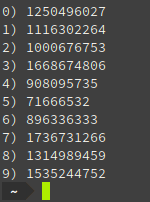
\includegraphics{lcg_output.png}
    \caption{Primeiros 10 números gerados a partir de 42}
    \label{fig:lcg_output}
\end{figure}

\section{Teste de primalidade de Fermat}

O teste de primalidade de Fermat é um teste probabilístico para determinar se
um número é provavelmente primo. Um número provavelmente primo é um inteiro que
satisfaz alguma condição específica que é satisfeita por todos os números que
são primos, mas não é satisfeita pela maioria dos números compostos
\cite{cormen:01}.

\subsection{Conceitos}

O teste é baseado no teorema de Fermat, que prova que para um primo $p$ tal que
$0 < a < p$, então $a^{p - 1} \equiv 1 \pmod{n}$.

Para testar se $p$ é primo, são escolhidos $a$s aleatórios no intervalo e
verifica-se se a equivalência prevalece. A probabilidade de que $p$ não seja
primo é cada vez mais baixa conforme mais valores de $a$ são testados.

Um número que não seja primo e passa no teste para uma base $a$ se chama
pseudoprimo de base $a$. De forma análoga, um número $a$ que acusa a composição
de um número é chamado de testemunha da composição de $a$.

Existe uma classe de números chamada de \textbf{números de Carmichael} que
satisfaz o teste de Fermat para todas as bases $a$ possíveis, mesmo não sendo
primos. Estes números são substancialmente mais raros do que números primos,
mas são suficientes para que o teste de Fermat não seja tão confiável quanto
outras alternativas.

\subsection{Exemplo}

Suponha que desejamos verificar se $p = 221$ é primo. Aleatoriamente se escolhe
uma base $1 < a < 221$, por exemplo, $a = 38$ e se aplica o teorema de Fermat:
\begin{center}
    $a^{n - 1} = 38^{220} \equiv 1 \pmod{221}$
\end{center}
Como a equivalência prevalece, ou $221$ é primo, ou é pseudoprimo para a base
$a = 38$. Aplicando o teorema com outra base, por exemplo, $a = 24$, podemos
verificar com mais precisão se $p$ é primo:
\begin{center}
    $a^{n - 1} = 24^{220} \equiv 81 \not\equiv \pmod{221}$
\end{center}
Conclui-se que $221$ não é primo e era apenas pseudoprimo de base $38$.

\subsection{Implementação}

O algoritmo do teste de Fermat foi implementado também em Python. O significado
das variáveis foi comentado ao lado das mesmas e os métodos devidamente
explicados. O teste é repetido de acordo com o parâmetro \texttt{tests}, por
padrão 20 vezes.

\lstinputlisting[language=Python]{fpt.py}

A parte relevante do algoritmo, a exponenciação modular ($a^{p - 1} \pmod{p}$)
é um método já embutido em várias linguagens, o que torna a implementação do
teste de primalidade de Fermat bastante simples.

Para gerar 10 números aleatoriamente e verificar com o teste de Fermat sua
primalidade pode ser usado o seguinte código:

\begin{lstlisting}[language=Python]
# for (i = 0; i < 10; ++i)
for i in range(10):
    rand = generator.rand()
    print("{0} primo? {1}".format(rand, fermat(rand)))
\end{lstlisting}

O gerador de números usado pelo teste de primalidade pode ser o mesmo gerador
usado para obter números. O resultado do código pode ser visto na
figura~\ref{fig:fpt_output}.

\begin{figure}[ht]
    \centering
    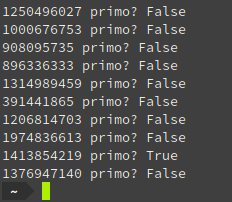
\includegraphics{fpt_output.png}
    \caption{10 números gerados e sua primalidade}
    \label{fig:fpt_output}
\end{figure}

\subsection{Comparação com Miller-Rabin}

Um outro teste de primalidade, o de Miller-Rabin (MR) também consiste em usar
uma propriedade que é verdadeira para todos os números primos e que não é
verdadeira para a maioria dos números compostos.

O algoritmo MR utiliza a um número primo $p$ e uma base $a$ qualquer, dado que
$1 < a < p$. $p - 1$ necessariamente é par e pode ser expresso na forma
$2^{s} \times d$, onde $s$ e $d$ são maiores que zero e $d$ é ímpar por
definição.

O teorema de MR afirma que, se $p$ é primo e $a$ não tem um divisor em comum
com $p$, então $a^{d} \equiv 1 \pmod{p}$ ou existe um
$r \in {0, 1, \ldots, s - 1}$ tal que $a^{2^{r} \times d} \equiv 1 \pmod{p}$.
Assim como no teste de Fermat, uma base $a$ que não satisfaz o teorema é
chamada de testemunha contra a primalidade de $p$.

O teste de MR é mais forte que o de Fermat porque ele não possui a falha de
não conseguir detectar os números de Carmichael, embora sua precisão seja a
mesma com os outros números. Ou seja, sua precisão é semelhante, mas não existe
um tipo de número "difícil" para o algoritmo de MR, o que o torna mais forte.

\section{Gerando números grandes}

Os parâmetros escolhidos pela maioria das implementações de LCGs não são
adequados para gerar números grandes o suficiente para aplicações
criptográficas, porque em geral são gerados números para representação em 32
ou 64 bits, e não 1024, 2048 ou 4096 como pode ser necessário para uso em
chaves criptográficas fortes.

Para gerar números grandes, é necessário alterar os parâmetros. Por exemplo, um
gerador para números de 4096 bits deve ter $m \geq 2^{4096}$ e é necessário
encontrar um $a$ e um $c$ que mantenham as relações definidas no
tópico~\ref{lcg:period}. Isso possui um custo computacional grande por usar
números de ordens de magnitude muito altas, de mais de mil dígitos decimais.

\subsection{Alternativa: escala de gerador menor}

Uma possibilidade é escalar os números de um gerador para números menores pela
proporção entre o módulo deste gerador e o módulo de um hipotético gerador para
números maiores (no exemplo, de 512 bits), como é feito no código abaixo:

\begin{lstlisting}[language=Python]
def rand512():
    rand = generator.rand() / generator.mod
    return rand * (2 ** 512)
\end{lstlisting}

Existe um custo adicional para converter o tipo de um número de inteiro para
decimal, e os dois fatores da divisão na linha 2 precisam ser convertidos para
que a operação seja efetuada, embora isso geralmente seja efetuado em tempo
constante.

Multiplicar por um número de tamanho arbitrário também não é uma operação
trivial: a complexidade da multiplicação na biblioteca GMP é da ordem de
$O(n^{k/(k - 2)})$, onde $n$ é a quantidade de dígitos e $k$ é relacionado com
o funcionamento interno do algoritmo.

A complexidade é, portanto, maior do que o próprio gerador, porém não afetada
pelo mesmo. Um número leva alguns milissegundos para ser gerado desta forma.

Onde \texttt{generator} é um gerador qualquer, podendo ser o citado nos
exemplos acima com $m = 2^{31}$. O que este código faz é transformar o inteiro
gerado $X_{n} \in [0, 2^{31})$ em um número decimal $Y_{n} \in [0, 1)$
proporcionalmente, e posteriormente multiplica pelo módulo desejado (neste
caso, $[0, 2^{512})$).

Essa alternativa requer que a linguagem também possua números decimais de
precisão arbitrária, já que é necessário transformar $m = 2^{512}$ em um
número decimal para efetuar a multiplicação. Em Python e na maioria das
linguagens, a precisão de números decimais vai até
$\approx 1.8 \times 10^{308}$, o que impossibilita o uso desta alternativa para
$m \geq 2^{1024}$.

Outro problema desta alternativa é que essencialmente é uma multiplicação dos
resultados de um gerador limitado, o que não aumenta a quantidade de possíveis
resultados. Ou seja, se escalado a partir de um gerador de $m = 2^{31}$, só
existirão $2^{31}$ possíveis números pseudoaleatórios, independente do tamanho
pelo qual será multiplicado.

\subsection{Alternativa: concatenando números menores}

Outra possibilidade é a de se gerar números de escala menor e concatenar até
que tenham o tamanho desejado. Utilizando gerador de números de 32 bits, seria
necessário concatenar números de 32 bits suficientes para formar um maior:

\begin{lstlisting}[language=Python]
def rand512():
    rand = 0  # inicializa como zero
    for i in range(512 / 32):  # executa 512/32 vezes
        # a linguagem precisa de suporte para numeros de tamanho arbitrario
        # e permitir operar logicamente sobre eles, para o shift left (<<)
        rand = (rand << 32) + generator.rand()
    return rand % (2 ** 512)
\end{lstlisting}

Essa alternativa é simples e o custo de calcular um número grande apenas muda
a constante da complexidade, e não a classe, portanto um número é gerado em
questão de milissegundos ou até menos.

O problema desta alternativa está no fato de que, para o LCG e outros geradores
cujo estado é o último número gerado, a sequência é sempre a mesma, e o período
fica menor na mesma proporção que o número fica maior.

No exemplo acima, são usados $2^{9} / 2^{5} = 2^{4} = 16$ números do gerador
para cada número grande. Na prática isso quer dizer que, se antes o ciclo tinha
período $2^{32}$, para gerar números grandes o período é reduzido para
$2^{32} / 2^{4} = 2^{28}$, o que é imprático para gerar uma grande quantidade
de números.

Uma boa heurística é que, se o algoritmo será usado para gerar $n$ números, ele
deve ter um período de pelo menos $n^{2}$ números \cite{malone:15}.
Se o algoritmo for usado para gerar chaves com mais de $2^{12}$ bits, essa
alternativa tem período de $2^{20}$ ($\approx$ 1 milhão), o que é
imprático dado que precisam ser gerados milhões de valores \textbf{diferentes}.

\subsection{Encontrando parâmetros melhores}

Para o LCG, encontrar parâmetros melhores que suportem geração de números
maiores é uma tarefa árdua, mas é a maneira mais plausível de se solucionar o
problema de gerar números grandes.

Para tal, é necessário fatorar o módulo $m$ e encontrar todos os seus divisores
para as duas primeiras regras, de que $c$ deve ser relativamente primo à $m$ e
de que $a - 1$ deve ser divisível por todos os fatores primos de $m$.

Encontrar todos os fatores primos de um número é extremamente custoso, já que
não há nenhum algoritmo eficiente, apenas força bruta. Um estudo conduzido em
2010 sugeriu que fatorar um inteiro de 1024 bits poderia levar mais de 2 mil
anos \cite{aoki:10}, portanto, não é prático encontrar novos fatores para um
LCG.

Além disso, como citado anteriormente, a necessidade de utilização de uma
biblioteca de números de tamanho árbitrário aumenta a complexidade da
manipulação destes primos grandes, o que faz com que gerar um número de
milhares de bits seja um processo mais custoso do que um número de 32 ou 64
bits.

\bibliographystyle{sbc/sbc}
\bibliography{lcg}

\end{document}
